\documentclass[12pt]{report}

% Import packages from local file
\usepackage{packages}


% Define the homework number as a variable
\newcommand{\HomeworkNumber}{2}

\begin{document}


% Add the cover


% Set up custom date format
\newdateformat{monthyeardate}{\monthname[\THEMONTH] \THEYEAR}

% Header and Footer configuration
\pagestyle{fancy}
\fancyhf{}
\fancyhead[L]{\leftmark}
\fancyhead[R]{\thepage}
\fancyfoot[C]{Probabilistic Modeling and Reasoning Homework \HomeworkNumber}

% Chapter and Section formatting
\titleformat{\chapter}[display]
  {\normalfont\bfseries}{}{0pt}{\Huge}
\titlespacing*{\chapter}{0pt}{-20pt}{20pt}

% Adjust header height and top margin
\setlength{\headheight}{14.49998pt}
\addtolength{\topmargin}{-2.49998pt}

% % Custom abstract environment
% \newenvironment{customabstract}
%   {\vspace*{1cm}
%    \begin{center}
%    \bfseries \huge Abstract
%    \end{center}
%    \vspace{0.5cm}
%    \normalfont \large}
%   {\vspace{1cm}}



\makeatletter
% Taken from http://ctan.org/pkg/centernot
\newcommand*{\centernot}{%
  \mathpalette\@centernot
}
\def\@centernot#1#2{%
  \mathrel{%
    \rlap{%
      \settowidth\dimen@{$\m@th#1{#2}$}%
      \kern.5\dimen@
      \settowidth\dimen@{$\m@th#1=$}%
      \kern-.5\dimen@
      $\m@th#1\not$%
    }%
    {#2}%
  }%
}
\makeatother


\begin{titlepage}
    \centering

    % University logo
    \vfill
    \includegraphics[width=0.3\textwidth]{UOMLOGOEN.eps}
    \vfill

    % Main title
    {\Huge \textbf{Probabilistic Modeling and Reasoning}} \\
    {\LARGE Homework — \HomeworkNumber}

    \vfill  % Vertical fill for dynamic centering
    % Authors' names
    {\Large \textbf{Nikolaos Liouliakis (AID25001)}} \\
    {\Large \textbf{Vasileios-Efraim Tsavalia (AID25006)}}

    % \vfill

    % % Course submission information
    % {\Large A report submitted for the course} \\
    % {\Large \textbf{Probabilistic Modeling and Reasoning}}

    \vfill

    % Program and University information
    {\Large MSc in Artificial Intelligence and Data Analytics} \\
    {\Large University of Macedonia}

    \vfill

    % Supervisor information
    {\Large \textbf{Supervisor: Professor Dimitris Christou-Varsakelis}}

    \vfill

    % Date with custom format
    {\Large \monthyeardate\today} % Automatically displays in "October 2024" format
    
\end{titlepage}


\newpage


\section*{Problem 1}

Details provided in the "README.txt" file.

\section*{Problem 2}

\begin{equation}    
 p(x,d,e,t,l,b,a,s) = p(d\mid e,b)p(b\mid s)p(x\mid e)p(e\mid t,l)p(l\mid s)p(t\mid a)p(a)p(s)
\end{equation}

\begin{equation}
    p(d) = \sum_{x,e,t,l,b,a,s \in \{0,1\}} p(x,d,e,t,l,b,a,s)
\end{equation}

\subsection*{Part 1}

\begin{equation*}
    p(d) = \sum_{x,e,t,l,b,a,s \in \{0,1\}} p(d\mid e,b)p(b\mid s)p(x\mid e)p(e\mid t,l)p(l\mid s)p(t\mid a)p(a)p(s)
\end{equation*}


\begin{align*}    
    p(d) = \sum_{x,e,t,l,b,s \in \{0,1\}}   p(d\mid e,b)p(b\mid s)p(x\mid e)p(e\mid t,l)p(l\mid s)p(t\mid a = 0)p(a = 0)p(s) + \\
                                p(d\mid e,b)p(b\mid s)p(x\mid e)p(e\mid t,l)p(l\mid s)p(t\mid a = 1)p(a = 1)p(s)
\end{align*}

% \begin{equation*}  
%     p(d) = \sum_{x,e,t,l,b,s \in \{0,1\}}   p(d\mid e,b)p(b\mid s)p(x\mid e)p(e\mid t,l)p(l\mid s)p(s) 
%     \Bigg( p(t\mid a = 0)p(a = 0) + p(t\mid a = 1)p(a = 1) \Bigg) 
% \end{equation*}


\begin{align*}  
    p(d) = \sum_{x,e,t,l,b,s \in \{0,1\}}   p(d\mid e,b)p(b\mid s)p(x\mid e)p(e\mid t,l)p(l\mid s)p(s) \cdot \\
    \Bigg( p(t\mid a = 0)p(a = 0) + p(t\mid a = 1)p(a = 1) \Bigg) 
\end{align*}



\begin{align*}    
    p(d) = \sum_{x,e,t,l,b,s \in \{0,1\}}   p(d\mid e,b)p(b\mid s)p(x\mid e)p(e\mid t,l)p(l\mid s)p(s)  \cdot \\
    \Bigg( p(t\mid a = 0)0.99 + p(t\mid a = 1)0.01 \Bigg)
\end{align*}




\begin{align*}    
    p(d) = \sum_{x,b,s \in \{0,1\}}  
        p(d\mid e=1,b)p(b\mid s)p(x\mid e=1)p(e=1\mid t=0,l=1)p(l=1\mid s)p(s) \\ \cdot \Bigg( p(t=0\mid a = 0)0.99 + p(t=0\mid a = 1)0.01 \Bigg) + \\
        p(d\mid e=1,b)p(b\mid s)p(x\mid e=1)p(e=1\mid t=1,l=0)p(l=0\mid s)p(s) \\ \cdot \Bigg( p(t=1\mid a = 0)0.99 + p(t=1\mid a = 1)0.01 \Bigg) + \\ 
        p(d\mid e=1,b)p(b\mid s)p(x\mid e=1)p(e=1\mid t=1,l=1)p(l=1\mid s)p(s) \\ \cdot \Bigg( p(t=1\mid a = 0)0.99 + p(t=1\mid a = 1)0.01 \Bigg) + \\
        p(d\mid e=0,b)p(b\mid s)p(x\mid e=0)p(e=0\mid t=0,l=0)p(l=0\mid s)p(s) \\ \cdot \Bigg( p(t=0\mid a = 0)0.99 + p(t=0\mid a = 1)0.01 \Bigg)
\end{align*}


\begin{align*}    
    p(d) = \sum_{x,b,s \in \{0,1\}}  
        p(d\mid e=1,b)p(b\mid s)p(x\mid e=1)p(l=1\mid s)p(s) \\ \cdot  \Bigg( p(t=0\mid a = 0) \cdot 0.99 + p(t=0\mid a = 1) \cdot 0.01 \Bigg) + \\
        p(d\mid e=1,b)p(b\mid s)p(x\mid e=1)p(l=0\mid s)p(s) \\ \cdot  \Bigg( p(t=1\mid a = 0) \cdot 0.99 + p(t=1\mid a = 1) \cdot 0.01 \Bigg) + \\ 
        p(d\mid e=1,b)p(b\mid s)p(x\mid e=1)p(l=1\mid s)p(s) \\ \cdot  \Bigg( p(t=1\mid a = 0) \cdot 0.99 + p(t=1\mid a = 1) \cdot 0.01 \Bigg) + \\
        p(d\mid e=0,b)p(b\mid s)p(x\mid e=0)p(l=0\mid s)p(s) \\ \cdot  \Bigg( p(t=0\mid a = 0) \cdot 0.99 + p(t=0\mid a = 1) \cdot 0.01 \Bigg)
\end{align*}





\begin{align*}    
    p(d) = \sum_{x,b,s \in \{0,1\}}  
        &p(d\mid e=1,b)p(b\mid s)p(x\mid e=1)p(l=1\mid s)p(s) \Bigg( 0.99 \cdot 0.99 + 0.95 \cdot 0.01 \Bigg) + \\
        &p(d\mid e=1,b)p(b\mid s)p(x\mid e=1)p(l=0\mid s)p(s) \Bigg( 0.01 \cdot 0.99 + 0.05 \cdot 0.01 \Bigg) + \\ 
        &p(d\mid e=1,b)p(b\mid s)p(x\mid e=1)p(l=1\mid s)p(s) \Bigg( 0.01 \cdot 0.99 + 0.05 \cdot 0.01 \Bigg) + \\
        &p(d\mid e=0,b)p(b\mid s)p(x\mid e=0)p(l=0\mid s)p(s) \Bigg( 0.99 \cdot 0.99 + 0.95 \cdot 0.01 \Bigg)
\end{align*}





\begin{align*}    
    p(d) = \sum_{x,b,s \in \{0,1\}}  
        &p(d\mid e=1,b)p(b\mid s)p(x\mid e=1)p(l=1\mid s)p(s) \cdot 0.9896 + \\
        &p(d\mid e=1,b)p(b\mid s)p(x\mid e=1)p(l=0\mid s)p(s) \cdot 0.0104 + \\ 
        &p(d\mid e=1,b)p(b\mid s)p(x\mid e=1)p(l=1\mid s)p(s) \cdot 0.0104 + \\
        &p(d\mid e=0,b)p(b\mid s)p(x\mid e=0)p(l=0\mid s)p(s) \cdot 0.9896
\end{align*}



\begin{align*}    
    p(d) = \sum_{x,b \in \{0,1\}}  
        &p(d\mid e=1,b)p(b\mid s=0)p(x\mid e=1)p(l=1\mid s=0)p(s=0) \cdot 0.9896 + \\
        &p(d\mid e=1,b)p(b\mid s=0)p(x\mid e=1)p(l=0\mid s=0)p(s=0) \cdot 0.0104 + \\ 
        &p(d\mid e=1,b)p(b\mid s=0)p(x\mid e=1)p(l=1\mid s=0)p(s=0) \cdot 0.0104 + \\
        &p(d\mid e=0,b)p(b\mid s=0)p(x\mid e=0)p(l=0\mid s=0)p(s=0) \cdot 0.9896 + \\        
        &p(d\mid e=1,b)p(b\mid s=1)p(x\mid e=1)p(l=1\mid s=1)p(s=1) \cdot 0.9896 + \\
        &p(d\mid e=1,b)p(b\mid s=1)p(x\mid e=1)p(l=0\mid s=1)p(s=1) \cdot 0.0104 + \\ 
        &p(d\mid e=1,b)p(b\mid s=1)p(x\mid e=1)p(l=1\mid s=1)p(s=1) \cdot 0.0104 + \\
        &p(d\mid e=0,b)p(b\mid s=1)p(x\mid e=0)p(l=0\mid s=1)p(s=1) \cdot 0.9896
\end{align*}

\begin{align*}    
    p(d) = \sum_{x,b \in \{0,1\}}  
        &p(d\mid e=1,b)p(b\mid s=0)p(x\mid e=1) \cdot 0.01 \cdot 0.5 \cdot 0.9896 + \\
        &p(d\mid e=1,b)p(b\mid s=0)p(x\mid e=1) \cdot 0.99 \cdot 0.5 \cdot 0.0104 + \\ 
        &p(d\mid e=1,b)p(b\mid s=0)p(x\mid e=1) \cdot 0.01 \cdot 0.5 \cdot 0.0104 + \\
        &p(d\mid e=0,b)p(b\mid s=0)p(x\mid e=0) \cdot 0.99 \cdot 0.5 \cdot 0.9896 + \\        
        &p(d\mid e=1,b)p(b\mid s=1)p(x\mid e=1) \cdot 0.1  \cdot 0.5 \cdot 0.9896 + \\
        &p(d\mid e=1,b)p(b\mid s=1)p(x\mid e=1) \cdot 0.9  \cdot 0.5 \cdot 0.0104 + \\ 
        &p(d\mid e=1,b)p(b\mid s=1)p(x\mid e=1) \cdot 0.1  \cdot 0.5 \cdot 0.0104 + \\
        &p(d\mid e=0,b)p(b\mid s=1)p(x\mid e=0) \cdot 0.9  \cdot 0.5 \cdot 0.9896
\end{align*}


\begin{align*}    
    p(d) = \sum_{x,b \in \{0,1\}}  
        &p(d\mid e=1,b)p(b\mid s=0)p(x\mid e=1) \cdot 0.004948 + \\
        &p(d\mid e=1,b)p(b\mid s=0)p(x\mid e=1) \cdot 0.005148 + \\ 
        &p(d\mid e=1,b)p(b\mid s=0)p(x\mid e=1) \cdot 0.000052 + \\
        &p(d\mid e=0,b)p(b\mid s=0)p(x\mid e=0) \cdot 0.489852 + \\        
        &p(d\mid e=1,b)p(b\mid s=1)p(x\mid e=1) \cdot 0.04948 + \\
        &p(d\mid e=1,b)p(b\mid s=1)p(x\mid e=1) \cdot 0.00468 + \\ 
        &p(d\mid e=1,b)p(b\mid s=1)p(x\mid e=1) \cdot 0.00052 + \\
        &p(d\mid e=0,b)p(b\mid s=1)p(x\mid e=0) \cdot 0.44532
\end{align*}


\begin{align*}    
    p(d) = \sum_{b \in \{0,1\}}  
        &p(d\mid e=1,b)p(b\mid s=0)p(x = 0 \mid e=1) \cdot 0.004948 + \\
        &p(d\mid e=1,b)p(b\mid s=0)p(x = 0 \mid e=1) \cdot 0.005148 + \\ 
        &p(d\mid e=1,b)p(b\mid s=0)p(x = 0 \mid e=1) \cdot 0.000052 + \\
        &p(d\mid e=0,b)p(b\mid s=0)p(x = 0 \mid e=0) \cdot 0.489852 + \\        
        &p(d\mid e=1,b)p(b\mid s=1)p(x = 0 \mid e=1) \cdot 0.04948 + \\
        &p(d\mid e=1,b)p(b\mid s=1)p(x = 0 \mid e=1) \cdot 0.00468 + \\ 
        &p(d\mid e=1,b)p(b\mid s=1)p(x = 0 \mid e=1) \cdot 0.00052 + \\
        &p(d\mid e=0,b)p(b\mid s=1)p(x = 0 \mid e=0) \cdot 0.44532 + \\
        &p(d\mid e=1,b)p(b\mid s=0)p(x = 1 \mid e=1) \cdot 0.004948 + \\
        &p(d\mid e=1,b)p(b\mid s=0)p(x = 1 \mid e=1) \cdot 0.005148 + \\ 
        &p(d\mid e=1,b)p(b\mid s=0)p(x = 1 \mid e=1) \cdot 0.000052 + \\
        &p(d\mid e=0,b)p(b\mid s=0)p(x = 1 \mid e=0) \cdot 0.489852 + \\        
        &p(d\mid e=1,b)p(b\mid s=1)p(x = 1 \mid e=1) \cdot 0.04948 + \\
        &p(d\mid e=1,b)p(b\mid s=1)p(x = 1 \mid e=1) \cdot 0.00468 + \\ 
        &p(d\mid e=1,b)p(b\mid s=1)p(x = 1 \mid e=1) \cdot 0.00052 + \\
        &p(d\mid e=0,b)p(b\mid s=1)p(x = 1 \mid e=0) \cdot 0.44532
\end{align*}


\begin{align*}    
    p(d) = \sum_{b \in \{0,1\}}  
        &p(d\mid e=1,b)p(b\mid s=0) \cdot  0.02 \cdot 0.004948 + \\
        &p(d\mid e=1,b)p(b\mid s=0) \cdot  0.02 \cdot 0.005148 + \\ 
        &p(d\mid e=1,b)p(b\mid s=0) \cdot  0.02 \cdot 0.000052 + \\
        &p(d\mid e=0,b)p(b\mid s=0) \cdot  0.95 \cdot 0.489852 + \\        
        &p(d\mid e=1,b)p(b\mid s=1) \cdot  0.02 \cdot 0.04948 + \\
        &p(d\mid e=1,b)p(b\mid s=1) \cdot  0.02 \cdot 0.00468 + \\ 
        &p(d\mid e=1,b)p(b\mid s=1) \cdot  0.02 \cdot 0.00052 + \\
        &p(d\mid e=0,b)p(b\mid s=1) \cdot  0.95 \cdot 0.44532 + \\
        &p(d\mid e=1,b)p(b\mid s=0) \cdot  0.98 \cdot 0.004948 + \\
        &p(d\mid e=1,b)p(b\mid s=0) \cdot  0.98 \cdot 0.005148 + \\ 
        &p(d\mid e=1,b)p(b\mid s=0) \cdot  0.98 \cdot 0.000052 + \\
        &p(d\mid e=0,b)p(b\mid s=0) \cdot  0.05 \cdot 0.489852 + \\        
        &p(d\mid e=1,b)p(b\mid s=1) \cdot  0.98 \cdot 0.04948 + \\
        &p(d\mid e=1,b)p(b\mid s=1) \cdot  0.98 \cdot 0.00468 + \\ 
        &p(d\mid e=1,b)p(b\mid s=1) \cdot  0.98 \cdot 0.00052 + \\
        &p(d\mid e=0,b)p(b\mid s=1) \cdot  0.05 \cdot 0.44532
\end{align*}


\begin{align*}    
    p(d) = 
    &p(d\mid e=1,b=0)p(b=0\mid s=0) \cdot  0.02 \cdot 0.004948 + \\
    &p(d\mid e=1,b=0)p(b=0\mid s=0) \cdot  0.02 \cdot 0.005148 + \\
    &p(d\mid e=1,b=0)p(b=0\mid s=0) \cdot  0.02 \cdot 0.000052 + \\
    &p(d\mid e=0,b=0)p(b=0\mid s=0) \cdot  0.95 \cdot 0.489852 + \\
    &p(d\mid e=1,b=0)p(b=0\mid s=1) \cdot  0.02 \cdot 0.04948  + \\
    &p(d\mid e=1,b=0)p(b=0\mid s=1) \cdot  0.02 \cdot 0.00468  + \\
    &p(d\mid e=1,b=0)p(b=0\mid s=1) \cdot  0.02 \cdot 0.00052  + \\
    &p(d\mid e=0,b=0)p(b=0\mid s=1) \cdot  0.95 \cdot 0.44532  + \\
    &p(d\mid e=1,b=0)p(b=0\mid s=0) \cdot  0.98 \cdot 0.004948 + \\
    &p(d\mid e=1,b=0)p(b=0\mid s=0) \cdot  0.98 \cdot 0.005148 + \\
    &p(d\mid e=1,b=0)p(b=0\mid s=0) \cdot  0.98 \cdot 0.000052 + \\
    &p(d\mid e=0,b=0)p(b=0\mid s=0) \cdot  0.05 \cdot 0.489852 + \\
    &p(d\mid e=1,b=0)p(b=0\mid s=1) \cdot  0.98 \cdot 0.04948  + \\
    &p(d\mid e=1,b=0)p(b=0\mid s=1) \cdot  0.98 \cdot 0.00468  + \\
    &p(d\mid e=1,b=0)p(b=0\mid s=1) \cdot  0.98 \cdot 0.00052  + \\
    &p(d\mid e=0,b=0)p(b=0\mid s=1) \cdot  0.05 \cdot 0.44532  + \\   
    &p(d\mid e=1,b=1)p(b=1\mid s=0) \cdot  0.02 \cdot 0.004948 + \\
    &p(d\mid e=1,b=1)p(b=1\mid s=0) \cdot  0.02 \cdot 0.005148 + \\
    &p(d\mid e=1,b=1)p(b=1\mid s=0) \cdot  0.02 \cdot 0.000052 + \\
    &p(d\mid e=0,b=1)p(b=1\mid s=0) \cdot  0.95 \cdot 0.489852 + \\
    &p(d\mid e=1,b=1)p(b=1\mid s=1) \cdot  0.02 \cdot 0.04948  + \\
    &p(d\mid e=1,b=1)p(b=1\mid s=1) \cdot  0.02 \cdot 0.00468  + \\
    &p(d\mid e=1,b=1)p(b=1\mid s=1) \cdot  0.02 \cdot 0.00052  + \\
    &p(d\mid e=0,b=1)p(b=1\mid s=1) \cdot  0.95 \cdot 0.44532  + \\
    &p(d\mid e=1,b=1)p(b=1\mid s=0) \cdot  0.98 \cdot 0.004948 + \\
    &p(d\mid e=1,b=1)p(b=1\mid s=0) \cdot  0.98 \cdot 0.005148 + \\
    &p(d\mid e=1,b=1)p(b=1\mid s=0) \cdot  0.98 \cdot 0.000052 + \\
    &p(d\mid e=0,b=1)p(b=1\mid s=0) \cdot  0.05 \cdot 0.489852 + \\
    &p(d\mid e=1,b=1)p(b=1\mid s=1) \cdot  0.98 \cdot 0.04948  + \\
    &p(d\mid e=1,b=1)p(b=1\mid s=1) \cdot  0.98 \cdot 0.00468  + \\
    &p(d\mid e=1,b=1)p(b=1\mid s=1) \cdot  0.98 \cdot 0.00052  + \\
    &p(d\mid e=0,b=1)p(b=1\mid s=1) \cdot  0.05 \cdot 0.44532
\end{align*}


\begin{align*}    
    p(d) = 
    & 0.7 \cdot 0.7 \cdot  0.02 \cdot 0.004948 + \\
    & 0.7 \cdot 0.7 \cdot  0.02 \cdot 0.005148 + \\
    & 0.7 \cdot 0.7 \cdot  0.02 \cdot 0.000052 + \\
    & 0.1 \cdot 0.7 \cdot  0.95 \cdot 0.489852 + \\
    & 0.7 \cdot 0.4 \cdot  0.02 \cdot 0.04948  + \\
    & 0.7 \cdot 0.4 \cdot  0.02 \cdot 0.00468  + \\
    & 0.7 \cdot 0.4 \cdot  0.02 \cdot 0.00052  + \\
    & 0.1 \cdot 0.4 \cdot  0.95 \cdot 0.44532  + \\
    & 0.7 \cdot 0.7 \cdot  0.98 \cdot 0.004948 + \\
    & 0.7 \cdot 0.7 \cdot  0.98 \cdot 0.005148 + \\
    & 0.7 \cdot 0.7 \cdot  0.98 \cdot 0.000052 + \\
    & 0.1 \cdot 0.7 \cdot  0.05 \cdot 0.489852 + \\
    & 0.7 \cdot 0.4 \cdot  0.98 \cdot 0.04948  + \\
    & 0.7 \cdot 0.4 \cdot  0.98 \cdot 0.00468  + \\
    & 0.7 \cdot 0.4 \cdot  0.98 \cdot 0.00052  + \\
    & 0.1 \cdot 0.4 \cdot  0.05 \cdot 0.44532  + \\   
    & 0.9 \cdot 0.3 \cdot  0.02 \cdot 0.004948 + \\
    & 0.9 \cdot 0.3 \cdot  0.02 \cdot 0.005148 + \\
    & 0.9 \cdot 0.3 \cdot  0.02 \cdot 0.000052 + \\
    & 0.8 \cdot 0.3 \cdot  0.95 \cdot 0.489852 + \\
    & 0.9 \cdot 0.6 \cdot  0.02 \cdot 0.04948  + \\
    & 0.9 \cdot 0.6 \cdot  0.02 \cdot 0.00468  + \\
    & 0.9 \cdot 0.6 \cdot  0.02 \cdot 0.00052  + \\
    & 0.8 \cdot 0.6 \cdot  0.95 \cdot 0.44532  + \\
    & 0.9 \cdot 0.3 \cdot  0.98 \cdot 0.004948 + \\
    & 0.9 \cdot 0.3 \cdot  0.98 \cdot 0.005148 + \\
    & 0.9 \cdot 0.3 \cdot  0.98 \cdot 0.000052 + \\
    & 0.8 \cdot 0.3 \cdot  0.05 \cdot 0.489852 + \\
    & 0.9 \cdot 0.6 \cdot  0.98 \cdot 0.04948  + \\
    & 0.9 \cdot 0.6 \cdot  0.98 \cdot 0.00468  + \\
    & 0.9 \cdot 0.6 \cdot  0.98 \cdot 0.00052  + \\
    & 0.8 \cdot 0.6 \cdot  0.05 \cdot 0.44532
\end{align*}


\begin{align*}    
    p(d) = 0.4359706
\end{align*}


\subsection*{Part 2}

\begin{equation}\label{eq:P2_p2}
    p(d=1 \mid s = 1) = \frac{p(d=1 , s = 1)}{p(s=1)}
\end{equation}


% \begin{equation}
%     p(d=1 \mid s = 1) = \frac{\sum_{x,e,t,l,b,a \in \{0,1\}} p(x,d=1,e,t,l,b,a,s=1)}{p(s=1)}
% \end{equation}

\begin{equation}
    p(d=1 , s = 1) = \sum_{x,e,t,l,b,a \in \{0,1\}} p(x,d=1,e,t,l,b,a,s=1)
\end{equation}

% \begin{equation}
%     p(d=1 , s = 0) = \sum_{x,e,t,l,b,a \in \{0,1\}} p(x,d=1,e,t,l,b,a,s=0)
% \end{equation}


\begin{align*}    
    p(d=1 , s = 1) = 
    &p(d=1\mid e=1,b=0)p(b=0\mid s=1) \cdot  0.02 \cdot 0.04948  + \\
    &p(d=1\mid e=1,b=0)p(b=0\mid s=1) \cdot  0.02 \cdot 0.00468  + \\
    &p(d=1\mid e=1,b=0)p(b=0\mid s=1) \cdot  0.02 \cdot 0.00052  + \\
    &p(d=1\mid e=0,b=0)p(b=0\mid s=1) \cdot  0.95 \cdot 0.44532  + \\
    &p(d=1\mid e=1,b=0)p(b=0\mid s=1) \cdot  0.98 \cdot 0.04948  + \\
    &p(d=1\mid e=1,b=0)p(b=0\mid s=1) \cdot  0.98 \cdot 0.00468  + \\
    &p(d=1\mid e=1,b=0)p(b=0\mid s=1) \cdot  0.98 \cdot 0.00052  + \\
    &p(d=1\mid e=0,b=0)p(b=0\mid s=1) \cdot  0.05 \cdot 0.44532  + \\  
    &p(d=1\mid e=1,b=1)p(b=1\mid s=1) \cdot  0.02 \cdot 0.04948  + \\
    &p(d=1\mid e=1,b=1)p(b=1\mid s=1) \cdot  0.02 \cdot 0.00468  + \\
    &p(d=1\mid e=1,b=1)p(b=1\mid s=1) \cdot  0.02 \cdot 0.00052  + \\
    &p(d=1\mid e=0,b=1)p(b=1\mid s=1) \cdot  0.95 \cdot 0.44532  + \\
    &p(d=1\mid e=1,b=1)p(b=1\mid s=1) \cdot  0.98 \cdot 0.04948  + \\
    &p(d=1\mid e=1,b=1)p(b=1\mid s=1) \cdot  0.98 \cdot 0.00468  + \\
    &p(d=1\mid e=1,b=1)p(b=1\mid s=1) \cdot  0.98 \cdot 0.00052  + \\
    &p(d=1\mid e=0,b=1)p(b=1\mid s=1) \cdot  0.05 \cdot 0.44532
\end{align*}




\begin{align*}    
    p(d=1 , s = 1) = 
    &0.7 0.4 \cdot  0.02 \cdot 0.04948  + \\
    &0.7 0.4 \cdot  0.02 \cdot 0.00468  + \\
    &0.7 0.4 \cdot  0.02 \cdot 0.00052  + \\
    &0.1 0.4 \cdot  0.95 \cdot 0.44532  + \\
    &0.7 0.4 \cdot  0.98 \cdot 0.04948  + \\
    &0.7 0.4 \cdot  0.98 \cdot 0.00468  + \\
    &0.7 0.4 \cdot  0.98 \cdot 0.00052  + \\
    &0.1 0.4 \cdot  0.05 \cdot 0.44532  + \\  
    &0.9  0.6 \cdot  0.02 \cdot 0.04948  + \\
    &0.9  0.6 \cdot  0.02 \cdot 0.00468  + \\
    &0.9  0.6 \cdot  0.02 \cdot 0.00052  + \\
    &0.8  0.6 \cdot  0.95 \cdot 0.44532  + \\
    &0.9  0.6 \cdot  0.98 \cdot 0.04948  + \\
    &0.9  0.6 \cdot  0.98 \cdot 0.00468  + \\
    &0.9  0.6 \cdot  0.98 \cdot 0.00052  + \\
    &0.8  0.6 \cdot  0.05 \cdot 0.44532
\end{align*}

\begin{align*}
    p(d=1, s = 1) = 0.276404
\end{align*}


Therefore, by substituting in equation \eqref{eq:P2_p2}:

\begin{align*}
    p(d=1 \mid s = 1) = \frac{0.276404}{0.5} = 0.552808
\end{align*}

\subsection*{Part 3}

\begin{equation} \label{eq:P2_p3}
    p(d=1 \mid s = 0) = \frac{p(d=1 , s = 0)}{p(s=0)}
\end{equation}

\begin{equation}
    p(d=1 , s = 0) = \sum_{x,e,t,l,b,a \in \{0,1\}} p(x,d=1,e,t,l,b,a,s=0)
\end{equation}


\begin{align*}    
    p(d=1,s=0) = 
    &p(d=1\mid e=1,b=0)p(b=0\mid s=0) \cdot  0.02 \cdot 0.004948 + \\
    &p(d=1\mid e=1,b=0)p(b=0\mid s=0) \cdot  0.02 \cdot 0.005148 + \\
    &p(d=1\mid e=1,b=0)p(b=0\mid s=0) \cdot  0.02 \cdot 0.000052 + \\
    &p(d=1\mid e=0,b=0)p(b=0\mid s=0) \cdot  0.95 \cdot 0.489852 + \\
    &p(d=1\mid e=1,b=0)p(b=0\mid s=0) \cdot  0.98 \cdot 0.004948 + \\
    &p(d=1\mid e=1,b=0)p(b=0\mid s=0) \cdot  0.98 \cdot 0.005148 + \\
    &p(d=1\mid e=1,b=0)p(b=0\mid s=0) \cdot  0.98 \cdot 0.000052 + \\
    &p(d=1\mid e=0,b=0)p(b=0\mid s=0) \cdot  0.05 \cdot 0.489852 + \\ 
    &p(d=1\mid e=1,b=1)p(b=1\mid s=0) \cdot  0.02 \cdot 0.004948 + \\
    &p(d=1\mid e=1,b=1)p(b=1\mid s=0) \cdot  0.02 \cdot 0.005148 + \\
    &p(d=1\mid e=1,b=1)p(b=1\mid s=0) \cdot  0.02 \cdot 0.000052 + \\
    &p(d=1\mid e=0,b=1)p(b=1\mid s=0) \cdot  0.95 \cdot 0.489852 + \\
    &p(d=1\mid e=1,b=1)p(b=1\mid s=0) \cdot  0.98 \cdot 0.004948 + \\
    &p(d=1\mid e=1,b=1)p(b=1\mid s=0) \cdot  0.98 \cdot 0.005148 + \\
    &p(d=1\mid e=1,b=1)p(b=1\mid s=0) \cdot  0.98 \cdot 0.000052 + \\
    &p(d=1\mid e=0,b=1)p(b=1\mid s=0) \cdot  0.05 \cdot 0.489852 + 
\end{align*}

\begin{align*}    
    p(d=1,s=0) = 
    &0.7 \cdot 0.7 \cdot  0.02 \cdot 0.004948 + \\
    &0.7 \cdot 0.7 \cdot  0.02 \cdot 0.005148 + \\
    &0.7 \cdot 0.7 \cdot  0.02 \cdot 0.000052 + \\
    &0.1 \cdot 0.7 \cdot  0.95 \cdot 0.489852 + \\
    &0.7 \cdot 0.7 \cdot  0.98 \cdot 0.004948 + \\
    &0.7 \cdot 0.7 \cdot  0.98 \cdot 0.005148 + \\
    &0.7 \cdot 0.7 \cdot  0.98 \cdot 0.000052 + \\
    &0.1 \cdot 0.7 \cdot  0.05 \cdot 0.489852 + \\ 
    &0.9 \cdot 0.3 \cdot  0.02 \cdot 0.004948 + \\
    &0.9 \cdot 0.3 \cdot  0.02 \cdot 0.005148 + \\
    &0.9 \cdot 0.3 \cdot  0.02 \cdot 0.000052 + \\
    &0.8 \cdot 0.3 \cdot  0.95 \cdot 0.489852 + \\
    &0.9 \cdot 0.3 \cdot  0.98 \cdot 0.004948 + \\
    &0.9 \cdot 0.3 \cdot  0.98 \cdot 0.005148 + \\
    &0.9 \cdot 0.3 \cdot  0.98 \cdot 0.000052 + \\
    &0.8 \cdot 0.3 \cdot  0.05 \cdot 0.489852 + 
\end{align*}
% =0.1595666
\begin{align*}    
    p(d = 1, s = 0) =  0.1595666
\end{align*}


Therefore, by substituting in equation \eqref{eq:P2_p3}:

\begin{align*}
    p(d=1 \mid s = 0) = \frac{0.1595666}{0.5} = 0.3191332
\end{align*}

\section*{Problem 3}

Examine the following independence relations from the Chest Clinic Bayesian network.

\subsection*{a) \(d \perp\!\!\!\perp s\) False}

Independence of Dyspnea (\(d\)) and Smoking (\(s\))  \(d \perp\!\!\!\perp s\).
% There are two paths between s and d.

\begin{itemize}
    \item \textbf{Path 1: s - b - d }   \\    
This path does not contain any colliders, therefore it is not blocked and \(d \not\perp\!\!\!\perp s\)
    \item \textbf{Path 2: s - l - e - d } \\    
This path also does not contain any colliders, therefore it is not blocked and \(d \not\perp\!\!\!\perp s\)
\end{itemize}

\subsection*{b) \(s \perp\!\!\!\perp a\) True }
Independence of Smoking (\(s\)) and Visiting Asia (\(a\))

\begin{itemize}
    \item \textbf{Path: s - l - e - t - a} \\
    This path is blocked by $e$ because it is a collider, neither $e$ nor any of its descendants is in the conditioning set. Therefore \(d \perp\!\!\!\perp a\)
\end{itemize}


\subsection*{c) \(s \perp\!\!\!\perp a \mid e \) False }
Conditional independence of Smoking (\(s\)) and Visiting Asia (\(a\)) given Either Tuberculosis or Lung Cancer (\(e\))

\begin{itemize}
    \item \textbf{Path: s - l - e - t - a} \\
     This path is not blocked by $e$ because it is a collider that is in the conditioning set. Therefore \(d \not\perp\!\!\!\perp a \mid e \)
\end{itemize}



\subsection*{d) \(s \perp\!\!\!\perp x \mid d\) False }
Conditional Independence of Smoking (\(s\)) and Positive X-ray (\(x\)) Given Dyspnea (\(d\))

\begin{itemize}
    \item \textbf{Path 1: s - l - e - x}   \\    
    This path does not contain any colliders, but it is  it is blocked by $d$, which is a descendant of $e$. This path cannot induce dependence. 
    \item \textbf{Path 2: s - b - d - e - x} \\    
    In this path $d$ is a collider, but because it is in the conditioning set it does not block the path. 
    Therefore \(d \not\perp\!\!\!\perp x \mid d\)
\end{itemize}


% \section*{Problem 3 wrong}




% \subsection*{Problem Description}

% In this document, we analyze a set of four independence relations within a Bayesian network context, specifically derived from the Chest Clinic example. The variables in question represent conditions related to respiratory diseases, their causes, and their diagnostic indicators. The problems to be analyzed are as follows:

% \begin{enumerate}
%     \item \textbf{Independence of Dyspnea (\(d\)) and Smoking (\(s\))}:
%     \begin{itemize}
%         \item We need to determine if \(d \perp\!\!\!\perp s\).
%         \item This independence relation can be mathematically expressed as:
%         \[
%         P(d, s) = P(d) \cdot P(s) \quad \text{or equivalently} \quad P(d | s) = P(d).
%         \]
%     \end{itemize}

%     \item \textbf{Independence of Smoking (\(s\)) and Visiting Asia (\(a\))}:
%     \begin{itemize}
%         \item We need to determine if \(s \perp\!\!\!\perp a\).
%         \item The mathematical condition for this independence is:
%         \[
%         P(s, a) = P(s) \cdot P(a) \quad \text{or equivalently} \quad P(s | a) = P(s).
%         \]
%     \end{itemize}

%     \item \textbf{Conditional independence of Smoking (\(s\)) and Visiting Asia (\(a\)) given Either Tuberculosis or Lung Cancer (\(e\))}:
%     \begin{itemize}
%         \item We need to determine if \(s \perp\!\!\!\perp a \mid e\).
%         \item This conditional independence can be expressed as:
%         \[
%         P(s, a | e) = P(s | e) \cdot P(a | e) \quad \text{or equivalently} \quad P(s | a, e) = P(s | e).
%         \]
%     \end{itemize}

%     \item \textbf{Conditional independence of Smoking (\(s\)) and Positive X-ray (\(x\)) given Dyspnea (\(d\))}:
%     \begin{itemize}
%         \item We need to determine if \(s \perp\!\!\!\perp x \mid d\).
%         \item The mathematical condition for this conditional independence is:
%         \[
%         P(s, x | d) = P(s | d) \cdot P(x | d) \quad \text{or equivalently} \quad P(x | s, d) = P(x | d).
%         \]
%     \end{itemize}
% \end{enumerate}


% \subsection*{General Methodology}

% The methodology for analyzing each of these problems consists of the following steps, aligned with the principles of structured reasoning and mathematical rigor:

% \subsection*{1. Interpreting Bayesian Networks}
% \begin{itemize}
%     \item Utilize the concept of \textbf{d-separation} to identify potential independence and conditional independence relations between variables.
%     \item Analyze graph paths to determine whether conditioning on specific nodes blocks or unblocks information flow.
% \end{itemize}

% \subsection*{2. Problem-Solving Approach}
% \begin{itemize}
%     \item \textbf{Path Analysis}: Identify all possible paths between the variables in question.
%     \item \textbf{Collider Identification}: Determine the presence of colliders and how conditioning on nodes affects dependency.
%     \item \textbf{Mathematical Formulation}: Use probability expressions to represent independence conditions.
%     \item \textbf{Verification}: Cross-verify results using alternative methods when applicable, ensuring consistency.
% \end{itemize}

% \subsection*{3. Verification and Validation}
% \begin{itemize}
%     \item Implement error analysis to consider any edge cases that might influence the conclusion.
%     \item Reflect on the results using a quality scoring system to indicate confidence in the solution.
% \end{itemize}

% \subsection{Solutions}

% \subsection*{Solution Outline}

% We will address each problem using the following structured steps:
% 1. **Identify the Nodes and Relationships**: We determine the direct connections between the variables in the Bayesian network.
% 2. **Check the Path**: We analyze the possible paths between the nodes to see if any connection is blocked.
% 3. **Evaluate Independence Using d-Separation**: Based on the path analysis, we apply the concept of d-separation to determine if the independence condition holds.

% Below, we will apply these steps to each of the four problems:

% \subsubsection*{Problem 1: Independence of Dyspnea (\(d\)) and Smoking (\(s\))}

% \begin{enumerate}
%     \item \textbf{Identify the Nodes and Relationships}:
%         - We observe that \(d\) (Dyspnea) is directly influenced by \(b\) (Bronchitis) and \(l\) (Lung Cancer), while \(s\) (Smoking) affects both \(b\) and \(l\).
%     \item \textbf{Check the Path}:
%         - There is a path from \(s\) to \(d\) through the nodes \(b\) and \(l\).
%     \item \textbf{Evaluate Independence Using d-Separation}:
%         - Since there is a connecting path through the common effect nodes (\(b\) and \(l\)), this path is not blocked. Therefore, we conclude that \(d\) is not independent of \(s\).
%     \item \textbf{Conclusion}:
%         - \(d \not\perp\!\!\!\perp s\) because the influence of smoking on dyspnea is mediated through bronchitis and lung cancer.
% \end{enumerate}

% \subsubsection*{Problem 2: Independence of Smoking (\(s\)) and Visiting Asia (\(a\))}

% \begin{enumerate}
%     \item \textbf{Identify the Nodes and Relationships}:
%         - \(s\) (Smoking) and \(a\) (Visiting Asia) are not directly connected, and they affect different parts of the network.
%     \item \textbf{Check the Path}:
%         - There is no direct or indirect path that connects \(s\) to \(a\) in the network.
%     \item \textbf{Evaluate Independence Using d-Separation}:
%         - Since there is no connecting path, we can say that the nodes are d-separated.
%     \item \textbf{Conclusion}:
%         - \(s \perp\!\!\!\perp a\), meaning that Smoking and Visiting Asia are independent.
% \end{enumerate}

% \subsubsection*{Problem 3: Conditional Independence of Smoking (\(s\)) and Visiting Asia (\(a\)) Given Either Tuberculosis or Lung Cancer (\(e\))}

% \begin{enumerate}
%     \item \textbf{Identify the Nodes and Relationships}:
%         - \(s\) and \(a\) both influence different conditions but converge at the node \(e\) (Either Tuberculosis or Lung Cancer).
%     \item \textbf{Check the Path}:
%         - There is a converging path at the node \(e\). When conditioning on \(e\), we need to check if this blocks the influence.
%     \item \textbf{Evaluate Independence Using d-Separation}:
%         - Conditioning on \(e\) means we focus on whether information from \(a\) changes the belief about \(s\) when \(e\) is known. Since \(e\) acts as a collider, it blocks the path unless both are explicitly conditioned on.
%     \item \textbf{Conclusion}:
%         - \(s \perp\!\!\!\perp a \mid e\), indicating that Smoking and Visiting Asia are conditionally independent given Either Tuberculosis or Lung Cancer.
% \end{enumerate}

% \subsubsection*{Problem 4: Conditional Independence of Smoking (\(s\)) and Positive X-ray (\(x\)) Given Dyspnea (\(d\))}

% \begin{enumerate}
%     \item \textbf{Identify the Nodes and Relationships}:
%         - The node \(x\) (Positive X-ray) is connected to the network through \(t\) (Tuberculosis) and \(l\) (Lung Cancer), while \(d\) (Dyspnea) is linked to \(l\) and \(b\) (Bronchitis), both influenced by Smoking.
%     \item \textbf{Check the Path}:
%         - The primary path from \(s\) to \(x\) involves passing through \(l\), which leads to \(d\), and then to \(x\).
%         - We need to examine if conditioning on \(d\) blocks this path.
%     \item \textbf{Evaluate Independence Using d-Separation}:
%         - Conditioning on \(d\) does block the path because it acts as an intermediate node (a chain structure) between \(l\) and \(x\), thereby preventing influence from \(s\) to \(x\).
%     \item \textbf{Conclusion}:
%         - \(s \perp\!\!\!\perp x \mid d\), meaning that Smoking and Positive X-ray are conditionally independent given Dyspnea.
% \end{enumerate}





\section*{Problem 4}


\begin{figure}[H]
    \centering
    \begin{minipage}{0.45\linewidth}
        \centering
        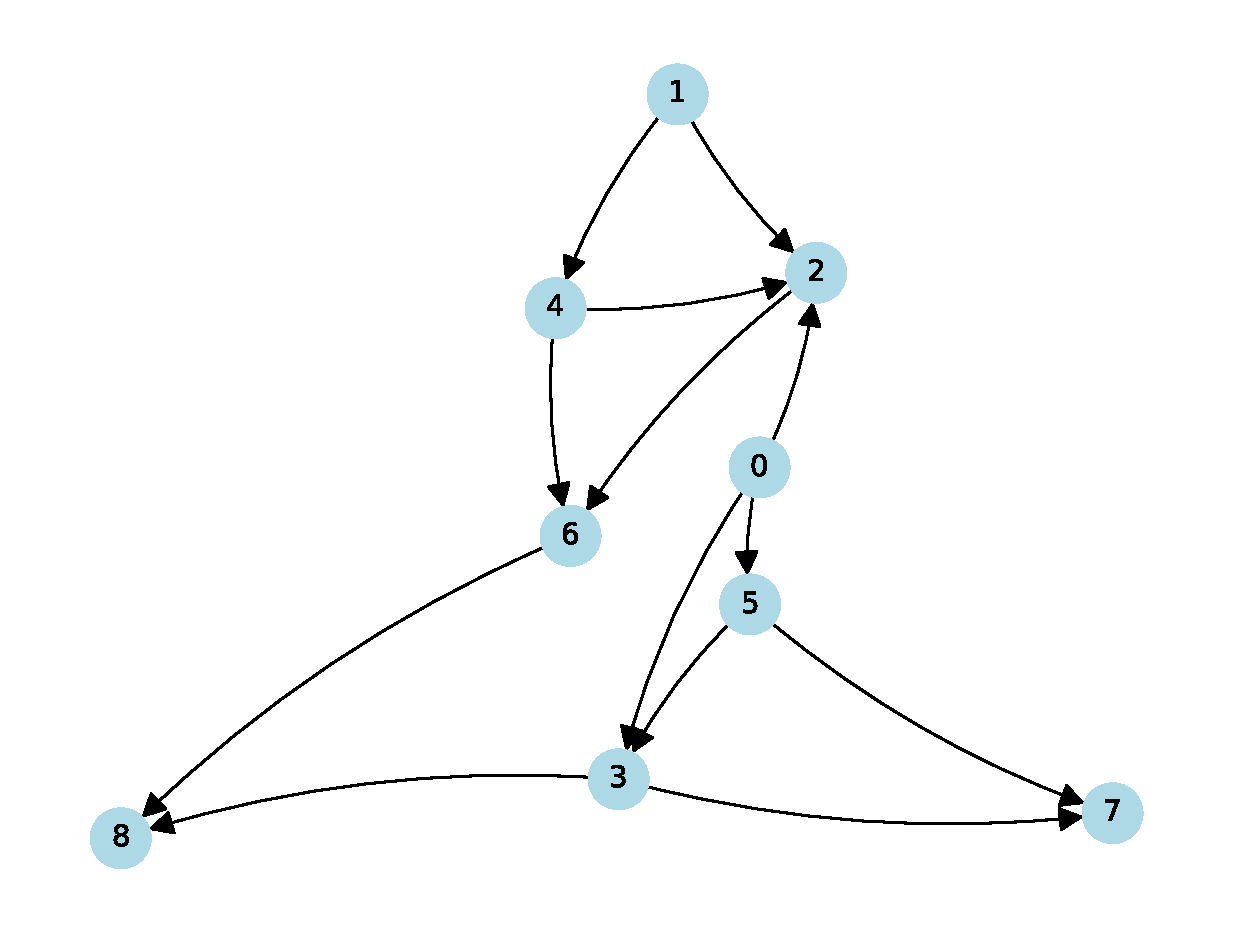
\includegraphics[width=\linewidth]{P4_graphA.eps}
        \caption{Belief network A}
    \end{minipage}%
    \hfill
    \begin{minipage}{0.45\linewidth}
        \centering
        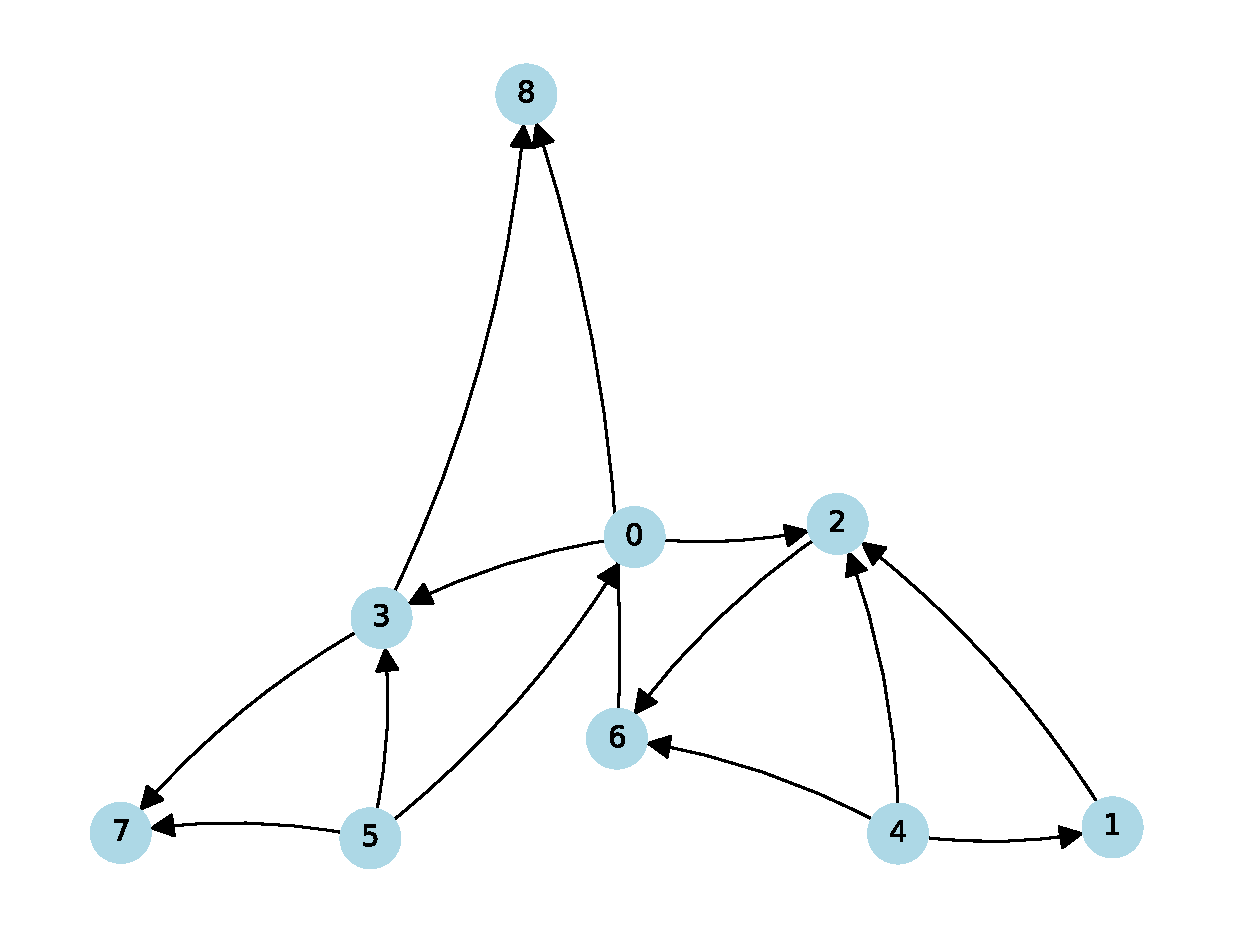
\includegraphics[width=\linewidth]{P4_graphB.eps}
        \caption{Belief network B}
    \end{minipage}
\end{figure}

The two belief networks are Markov equivalent.

% The two belief networks are not Markov equivalent due to immorality mismatch.

% The two belief networks are not Markov equivalent due to skeleton mismatch.




% \section*{Description}
% We are tasked with determining whether two belief networks (Bayesian networks) represented by directed acyclic graphs (DAGs) are Markov equivalent. Markov equivalence between two belief networks means that both networks encode the same set of conditional independence relations. Mathematically, two DAGs are Markov equivalent if and only if:
% \begin{itemize}
%     \item They have the same \textit{skeleton} (i.e., the underlying undirected graph obtained by ignoring edge directions).
%     \item They have the same set of \textit{immoralities} (also called v-structures), which occur when two parent nodes of a common child are not directly connected.
% \end{itemize}
% The goal is to build a function that, given two adjacency matrices, checks whether the corresponding belief networks are Markov equivalent. If they are not equivalent, we need to report whether the issue lies with the skeleton or the set of immoralities.

% \section*{Methodology}
% \subsection*{1. Skeleton Equivalence}
% The first step in checking Markov equivalence is to ensure that both graphs have the same skeleton. The skeleton of a DAG is the undirected version of the graph, obtained by ignoring the direction of edges. To determine whether two skeletons are equivalent, we can represent each DAG as an adjacency matrix, convert these matrices to undirected graphs, and compare them. Mathematically, if the adjacency matrices are \( A \) and \( B \), we need to:
% \[
% G_A = \text{Undirected version of DAG from } A
% \]
% \[
% G_B = \text{Undirected version of DAG from } B
% \]
% If \( G_A \) and \( G_B \) are isomorphic, the skeletons are equivalent.

% \subsection*{2. Identifying Immoralities}
% Immoralities in a DAG are configurations where two parent nodes of a common child are not connected by an edge. Formally, for a node \( X_k \), if nodes \( X_i \) and \( X_j \) are both parents of \( X_k \) (i.e., there are directed edges from \( X_i \rightarrow X_k \) and \( X_j \rightarrow X_k \)) and \( X_i \) and \( X_j \) are not directly connected, then \( (X_i, X_j, X_k) \) forms an immorality. 

% To check whether two graphs have the same set of immoralities, we need to:
% \begin{itemize}
%     \item For each node \( X_k \), find all pairs of parent nodes \( X_i \) and \( X_j \).
%     \item Check whether the parents \( X_i \) and \( X_j \) are not directly connected.
%     \item Record the set of all immoralities for both networks.
% \end{itemize}
% If the sets of immoralities for both networks match, then they are Markov equivalent in terms of immoralities.

% \section*{Solution Outline}
% \subsection*{Step 1: Read and Parse the Adjacency Matrices}
% We first read the adjacency matrices representing the two belief networks. These matrices can be read from text files, where each file contains a space-separated list of 0s and 1s representing the edges between nodes.

% \subsection*{Step 2: Check Skeleton Equivalence}
% Using a graph library (e.g., \texttt{networkx} in Python), we convert the adjacency matrices into undirected graphs. This can be done by treating the matrix as an undirected graph and ignoring the direction of edges. We then check whether these undirected graphs are isomorphic. If they are not, the two networks are not Markov equivalent, and we report a skeleton mismatch.

% \subsection*{Step 3: Identify and Compare Immoralities}
% For each graph, we identify the set of immoralities by iterating over all nodes. For each node \( X_k \), we find all pairs of parents and check whether the parents are connected. If the parents are not connected, we add this configuration to the set of immoralities. After identifying the sets of immoralities for both networks, we compare them. If they do not match, we report an immorality mismatch.

% \subsection*{Step 4: Return the Result}
% If both the skeletons and the sets of immoralities match, we conclude that the two belief networks are Markov equivalent. Otherwise, we return a message specifying whether the mismatch was due to the skeleton or the set of immoralities.





\section*{Problem 5}

\begin{figure}[H]
    \centering
    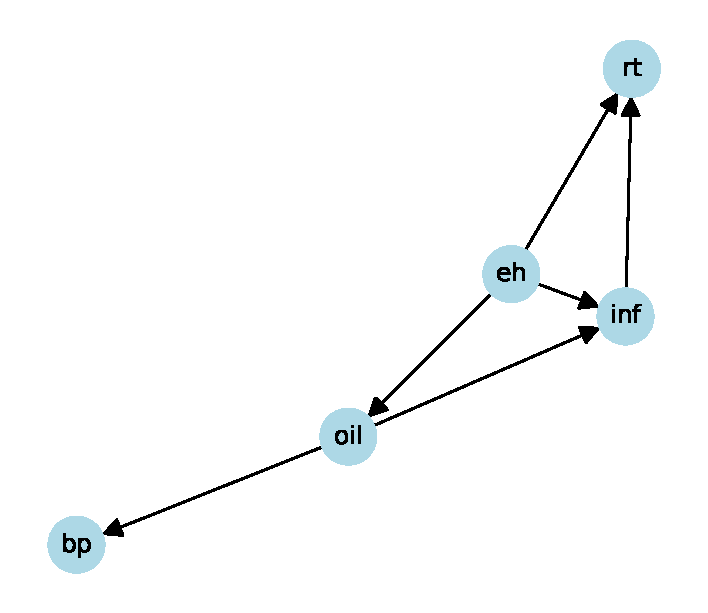
\includegraphics[width=0.65\linewidth]{P5_graph.eps}%
    \caption{Belief network that models the relation between the variables oil, inf, eh, bp, rt.}
\end{figure}



\end{document}
